\section{Evaluation}
\label{sec:evaluation}
% describe systems:
We performed an empirical evaluation of \sys to determine how it
compares to existing solvers for recursion-free CHC systems.
%
To do so, we implemented \sys as a modification of \duality CHC
solver, which is included in the \zthree theorem prover~\cite{z3}.
%
We modified \duality to use \sys as its solver for recursion-free CHC
systems.
%
We modified the algorithm used by \duality to generate recursion-free
unwindings of a given recursive system so that in each iteration, it
generates an unwinding with a maximal set of relational predicates and
clauses.
%
In the following context, ``\sys'' refers to \duality modified to
solve general CHC systems.

% describe benchmarks:
We evaluated \sys and \duality on 4,309 CHC systems generated from
programs in the SV-COMP 2015~\cite{svcomp15} verification benchmark
suite.
%
To generate CHC systems, we ran the \seahorn~\cite{gurfinkel15}
verification framework with its default settings (procedures are not
inlined and each loop-free fragment is a clause), set to timeout at 90
seconds.
%
We used the benchmarks in SV-COMP 2015~\cite{svcomp15} because they
were used to evaluate \duality in previous work~\cite{mcmillan14}.

We also attempted to compare \sys to the \eldarica CHC solver, but
\eldarica could not parse the CHC systems generated by \seahorn.
%
We compared \sys and \eldarica on an alternative set of benchmarks
generated by the UFO model checker~\cite{albarghouthi12c}, and found
that \sys outperformed \eldarica by at least an order of magnitude on
an overwhelming number of cases.
%
As a result, we focus our discussion on a comparison of \sys and
\duality.

% experimental setups:
All experiments were run using a single thread 
on a machine with 16 1.4 GHz processors and
128 GB of RAM.
%
We ran the solvers on each benchmark, timing out each implementation
after 180 seconds.

% summarize the result
Out of 4,309 benchmarks, \sys solved or refuted 2,408 while \duality
solved or refuted 2,321. \sys timed out on 762 benchmarks and \duality
timed out on 1,145.
%
On the remaining benchmarks, some constraint caused \zthree's
interpolating theorem prover to fail, meaning the result was neither a
solve nor a refutation. \sys reached this failure on 1,139 benchmarks
while \duality failed on 843.
%
The two solvers can induce a failure in \zthree on different systems
because in attempting to solve a given system, they generate different
interpolation queries.


\begin{figure}[t]
  \centering
  \begin{floatrow}[2]
    \ffigbox[.48\textwidth] %
    {\caption{Solving times of \sys vs. \duality.
        %
        The $x$ and $y$ axes range over the solving times in seconds
        of \sys and \duality, respectively.
        %
        Each point depicts the performance of a benchmark.
        %
        The line $y = x$ is shown in red.} %
      \label{fig:complete-data} }
    { 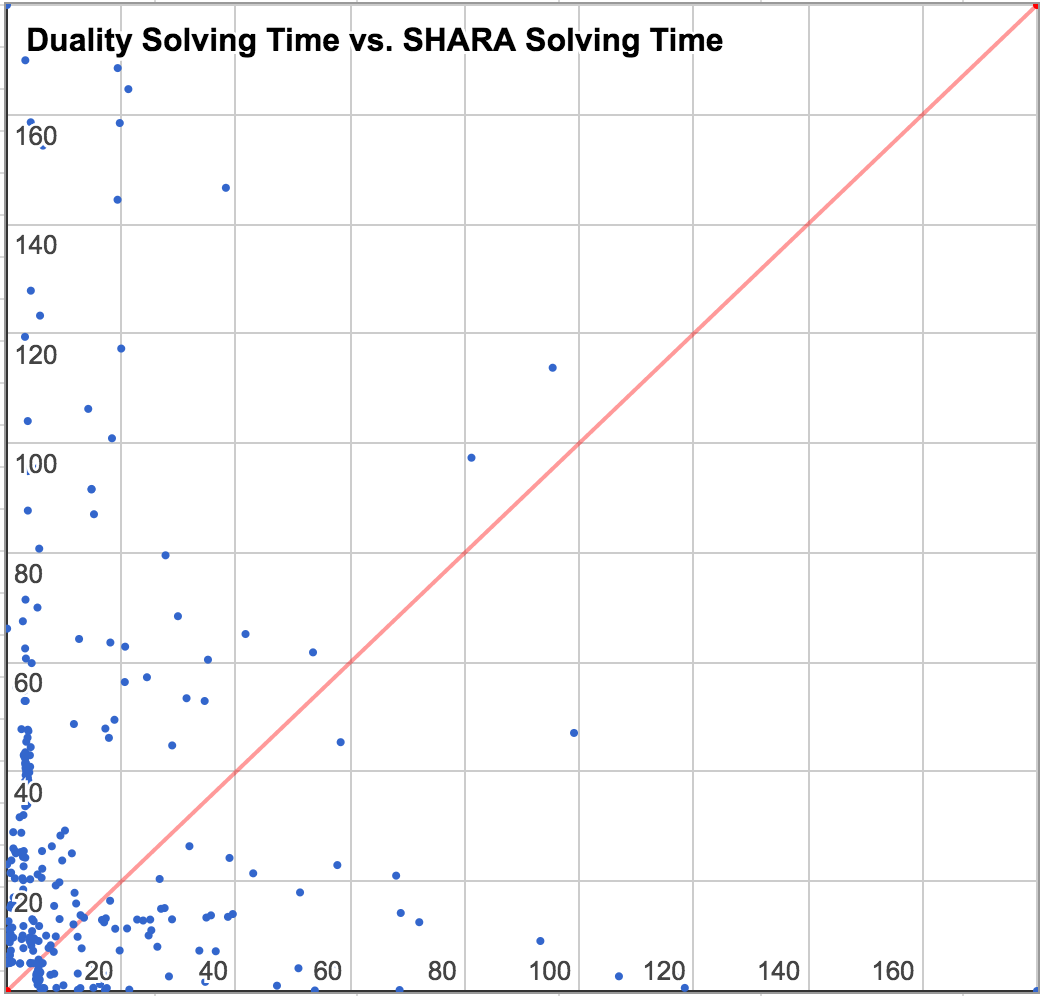
\includegraphics[width=\linewidth]{fig/complete.png} }
    %
    \ffigbox[.48\textwidth] %
    { \caption{Times of \sys and \duality vs. system size.
        %
        The $x$-axis ranges over the size of a given system, and the
        $y$-axis ranges over solvers' times.
        %
        Measurements of \sys and \duality are shown in blue and
        red, respectively. } %
      \label{fig:size} }
     { 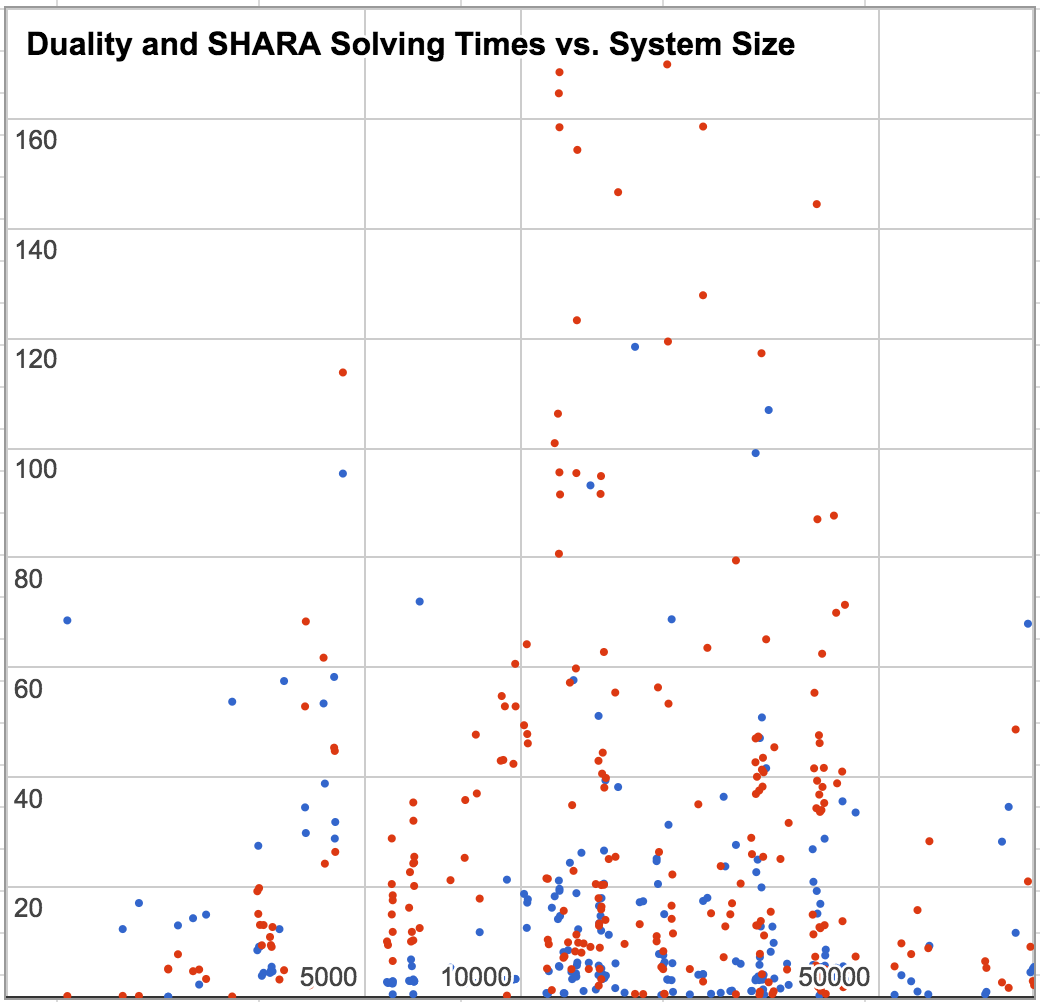
\includegraphics[width=\linewidth]{fig/size.png} }
  \end{floatrow}
\end{figure}
% introduce figure, summarize data not included:
The results of our evaluation are shown in
\autoref{fig:complete-data}.
%
Of the 4,040 benchmarks on which both solvers took a short amount
of time---less than five seconds---\sys solved the benchmarks in an
average of 0.51 seconds and \duality solved them in an average of 0.42
seconds.
%
\autoref{fig:complete-data} contains data for benchmarks which took
longer than five second for both systems to solve.
%
Out of these 269 benchmarks, \sys solved 185 in less time
than \duality, and solved 159 in less than half the time of \duality.
%
\duality solved 84 in less time than \sys, and solved 53 in less than
half the time of \sys.
%
Of the 762 benchmarks on which \sys timed out, \duality solved or
found a counterexample to 185.
%
Of the 1,145 benchmarks on which \duality timed out, \sys solved or
found a counterexample to 470.

% analyze data on system size:
\autoref{fig:size} shows the relationship between the solving times of
\duality and \sys and the size of a given system, measured as lines of
code in the format generated by \seahorn.
%
The majority of files have between 1,000 and 100,000 lines, so
\autoref{fig:size} is restricted to this range.
%
The data indicates that that performance improvement of \sys compared
to \duality is consistent across systems of all sizes available.

%result is good
The results indicate that \textbf{(1)} on a significant number of
different verification problems, \sys can perform significantly better than
\duality, but
%
\textbf{(2)} there are some cases in which the strengths of each
algorithm yield better results.
%
We collected the differences between sizes of a given system and its
minimal CDD expansion generated by \sys and found that they were
independent of \sys's performance compared to \duality.
%
Thus, while \duality may in the worst case enumerate exponentially
many derivation trees, it appears to enumerate far fewer
than the worst-case bound in some cases, causing it to perform better
than \sys.
%
Our results indicate that a third approach that combines the strengths
of both \duality and \sys, perhaps by lazily unwinding a given
recursion-free system into a series of CDD systems instead of
derivation trees, could yield further improvements.

%%% Local Variables: 
%%% mode: latex
%%% TeX-master: "p"
%%% End: 
